\section{Recap: Attention in Seq2Seq}
\begin{frame}{The Attention Mechanism (Recap)}
  \centering
  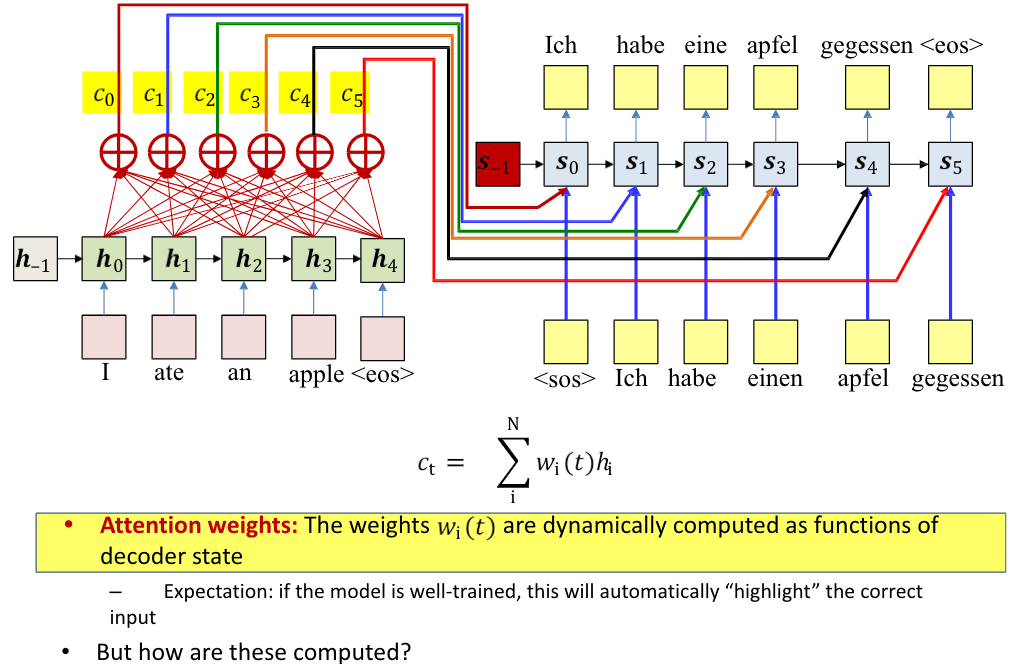
\includegraphics[width=0.45\paperwidth, height=0.45\paperheight, keepaspectratio]{images/attention-deep-dive/attention_dynamic_weights_decoder.png}

  \begin{itemize}
    \item The decoder builds a fresh context vector at every step: $c_t = \sum_i w_i(t)\, h_i$, a weighted sum of all encoder states, not the hidden state of any single input word.
    \item The weights $w_i(t)$ are computed dynamically from the previous decoder state $s_{t-1}$, are non-negative, and sum to one (softmax over scores).
    \item The scores behind these weights come from an alignment function, covered next.
  \end{itemize}
\end{frame}
